\subsection{The Capacitive Chair}
\begin{figure}[h]
\centering
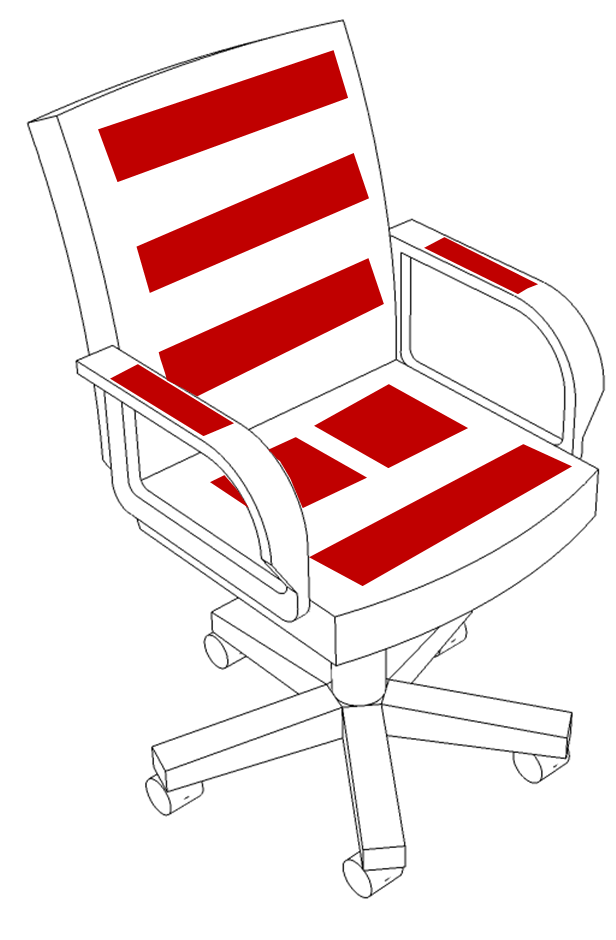
\includegraphics[width=0.4\textwidth]{images/smartofficechair}
\caption{Smart office chair sketch - eight electrodes three in backrest, three on seat and two in armrests}
\label{fig:smartchair_sketch}
\end{figure}
The Capacitive Chair is a regular office chair equipped with eight capacitive proximity sensors that can detect different sitting postures and work-related stress levels by examining movement and breathing rate, developed in collaboration with Sebastian Frank \cite{Braun2013ChairAid}. Seven solid copper electrodes that are placed below the covering are augmented by a single conductive thread electrode that is placed in a mesh on the backrest. In the past smart chairs have used pressure sensors to infer posture and occupation \cite{tan2001sensing}. Combining presence and proximity sensing it is possible to directly infer postures where parts of the body do not touch the surface, e.g. if the body is arched towards the front, or if an arm is raised from the armrests. Additionally higher area electrodes in the backrest allow detecting the breathing rate by measuring the movement of the chest.

The Capacitive Chair aims at providing different services to a typical office worker and office managers. Using the occupation detection it is possible to advise for some type of physical activity, if the time spent in front of the screen was too long. The system can also advise the user to change to a more back-friendly posture or regularly switch the stance to achieve a more general workout. Using the breathing rate detection we are able to get some sort of measure of the current stress level associated to the given working situation. By adapting the environment it is possible to improve the working atmosphere and reduce stress. The Capacitive Chair uses a multifaceted data processing approach. A machine learning algorithm is associating the sensing data to one of nine different typical sitting positions, inspired by a recent study of sitting positions for modern device usage \cite{globalPosture}. An adaptive body model that is fitted to the current sensor values allows for fine grained adaptation of those postures. Finally a combination of Fourier and data variation analysis is calculating the current breathing rate \cite{Braun2013ChairAid}.

\subsubsection{Capacitive layout}
\begin{minipage}{\linewidth}
\centering
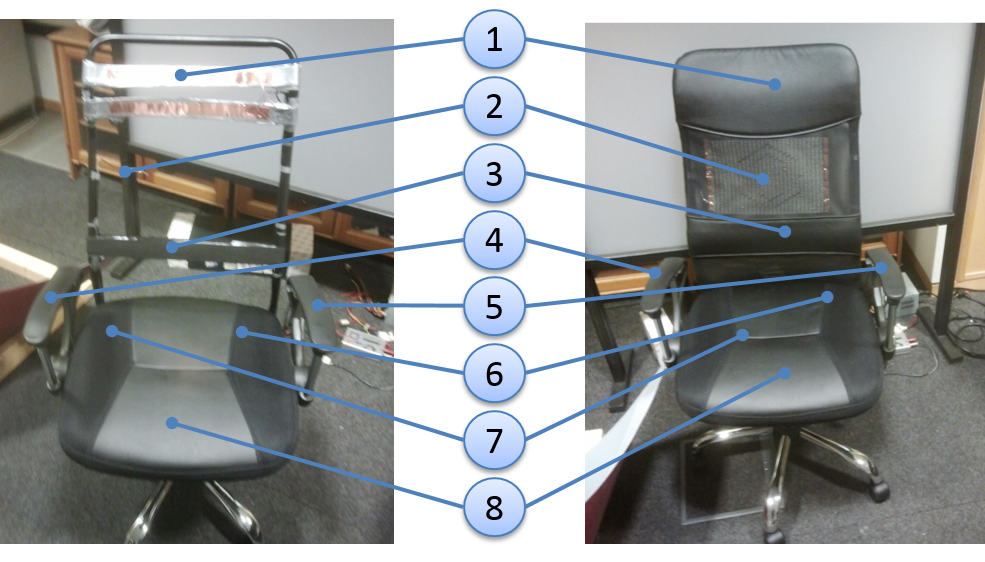
\includegraphics[width=0.8\textwidth]{images/prot_capchair_electrode_layout}
\captionof{figure}{Capacitive Chair electrode positions}
\label{fig:prot_capchair_electrode_layout}
\end{minipage}

The Capacitive Chair is based on a single OpenCapSense board that supports eight different electrodes. In order to get the posture measurements we need to distribute the electrodes equally on the different areas of the seat. The measurement of the breathing rate requires a larger electrode near the chest area. Consequently the electrodes are placed as follows:
\begin{enumerate}
\item Electrode on the upper part of the backrest (covered by faux leather)
\item Electrode in the central part of the backrest (using conductive thread)
\item Electrode in the lower part of the backrest (covered by faux leather)
\item Electrode below the right armrest
\item Electrode below the left armrest
\item Electrode for the left hip area below the left part of the seat
\item Electrode for the right hip area below the right part of the seat
\item Electrode for detecting both legs below the front part of the seat
\end{enumerate}

\begin{minipage}{\linewidth}
\centering
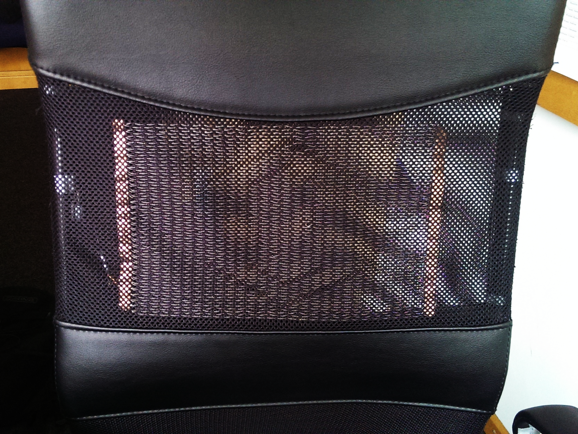
\includegraphics[width=0.8\textwidth]{images/prot_capchair_threadelectrode}
\captionof{figure}{Detail view of conductive thread electrode}
\label{fig:prot_capchair_threadelectrode}
\end{minipage}

The electrode in the central part of the backrest is based on conductive thread that was woven through the mesh material of the Capacitive Chair. The ends of the thread were connected to each other using conductive copper foil, in order to avoid negative effects that can occur when a single long electrode is used. A detail view is provided in Figure \ref{fig:prot_capchair_threadelectrode}.
 
\subsubsection{Processing}
The first steps of data processing are filtering using an 8-sample median filter and a baseline calibration for all channels. Additionally there is a dynamic normalization based on updated minimum and maximum values. For further processing we additionally need information about short-term value variance that we gather by calculating the difference quotient using a sample of ten average filtered measurements. Afterwards a FFT transformation is performed every $40ms$ discretized into 512 values. A binning operation is performed to look for significant signals in a reasonable frequency interval (0.1Hz-3Hz) to detect the most significant frequency associated to the breathing rate. 

\begin{minipage}{\linewidth}
\centering
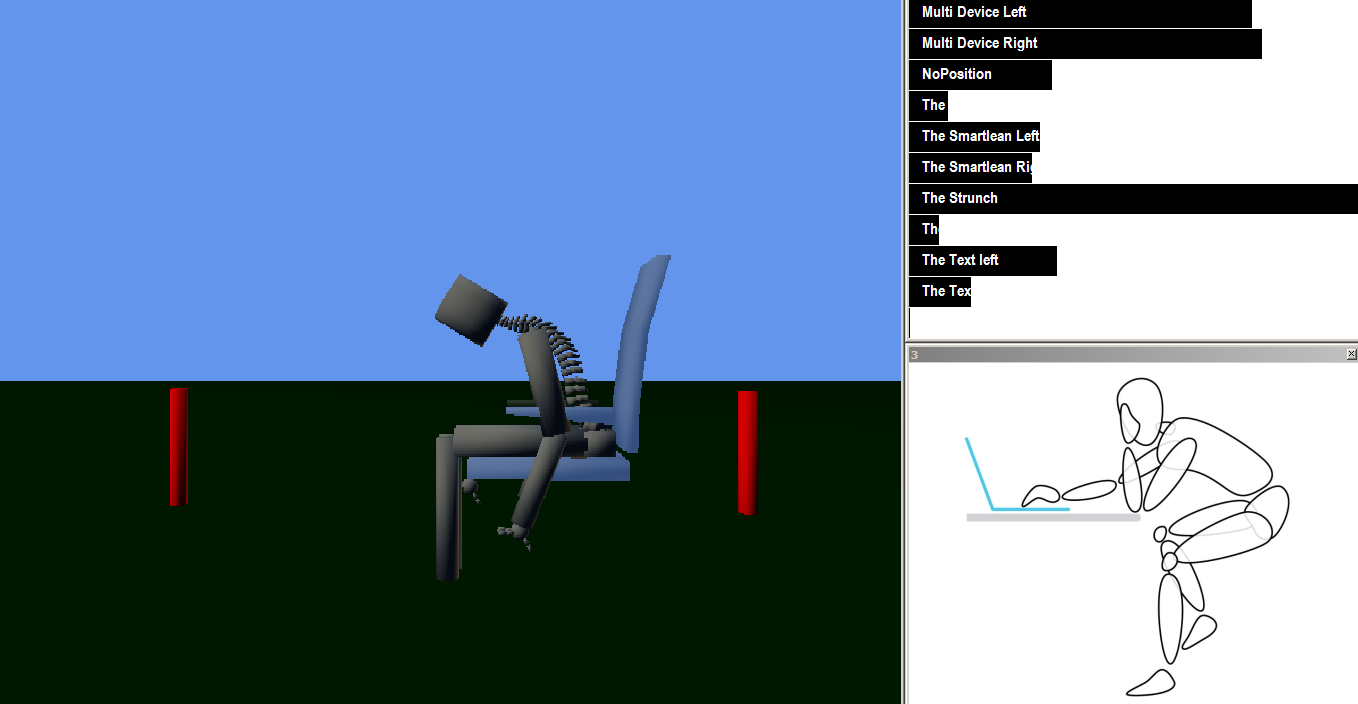
\includegraphics[width=0.9\textwidth]{images/smartchair_software}
\captionof{figure}{Screenshot of the Capacitive Chair application showing the fitted 3D model on the left, posture detection on the upper right and the recognized posture on the lower right}
\label{fig:smartchair_posture_software}
\end{minipage}

The method to calculate poses has been described in detail in Section \ref{ch:proc_model}. The processed values of all sensors are compared to previously trained sitting positions of a user. The result of this process in the created demonstration software is shown in Figure \ref{fig:smartchair_software}. The fine skeleton model output is shown on the left, the static gesture classification probabilities on the top right and a visualization of the resulting posture on the bottom right.

\begin{minipage}{\linewidth}
\centering

\includegraphics[width=0.7\textwidth]{images/placeholder}
\captionof{figure}{Screenshot of the Capacitive Chair application showing the fitted 3D model on the left, posture detection on the upper right and the recognized posture on the lower right}
\label{fig:smartchair_breathing_software}
\end{minipage}

Figure \ref{fig:smartchair_breathing_software} shows a screenshot of the demonstration software currently performing breathing rate detection. On the left side are the results of the FFT detection, showing the part of the signal relevant and the translation of the frequency to respirations per minute. ON the right there is the curve of sensor values showing the sinusoidal characteristics of the response to chest movement.

\subsubsection*{Distinguish work activity levels}
\begin{minipage}{\linewidth}
\centering
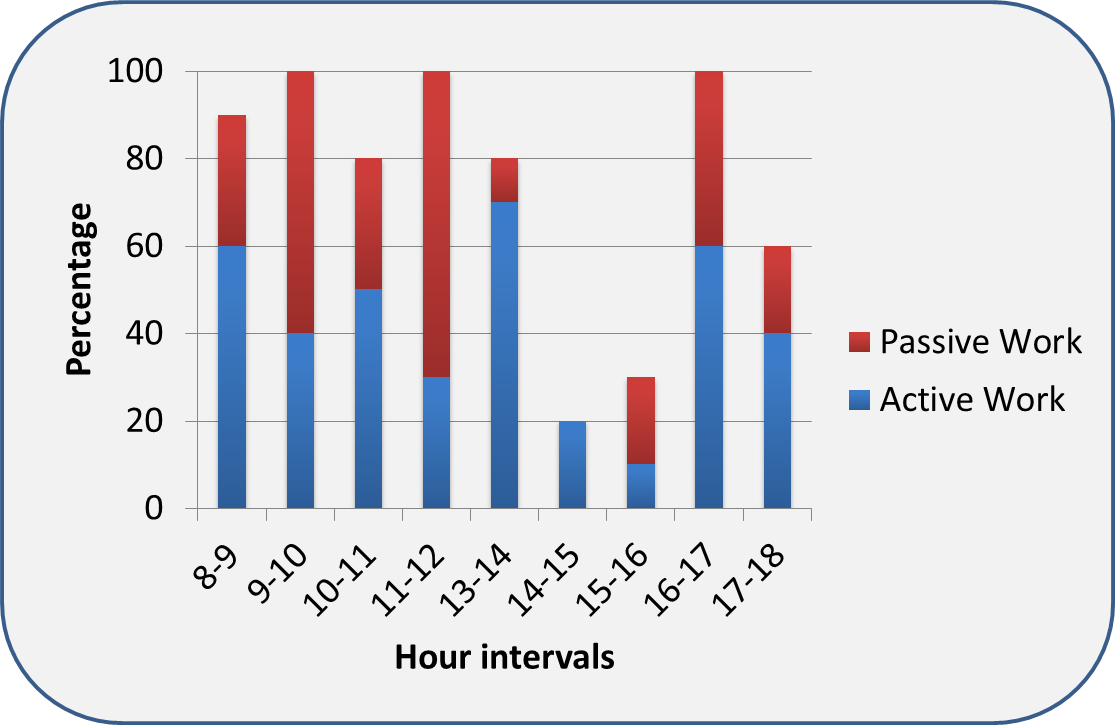
\includegraphics[width=0.6\textwidth]{images/smartchair_workact}
\captionof{figure}{ Work Activity aggregation over a single work day (mock-up)}
\label{fig:smartchair_workact}
\end{minipage}
An additional feature of the software developed for an EIT ICT Labs project, called Cognitive Endurance during 2013 is a recognition module for working activities throughout a day. The method works similar to the sleep phase recognition described in Section \ref{ch:proc_physio}. Aggregated sensor values are grouped into three potential activities, based on their variance over a certain amount of time.
\begin{itemize}
\item Active work as indicated by a certain level of movement while on the chair, e.g. gesturing while doing a phone call or performing small exercises
\item Passive work as being present on the chair while not moving a lot, e.g. reading a web page or writing a document
\item Not present at desk, whereas no one is currently sitting on the chair.
\end{itemize}

This results in an activity graph as shown in Figure \ref{fig:smartchair_workact} that creates an activity profile over the working day and can augment other activity tracking systems or act as self-standing system giving employers and employees feedback on the type and quality of work.

\subsubsection{Evaluation}
The Capacitive Chair was evaluated in two distinct studies. The first aimed at testing the aggregated recognition of working activities with several persons over various days. The second study was testing the posture recognition with various users that were additionally queried about their general impression of the system. In this section we are presenting results of both studies.
\subsubsection*{Working situation recognition}
The sensing chair supports distinguishing two different working situations that are determined using the method described in the previous section. The system also supports sending to the Cognitive Endurance server.
 
Figure \ref{fig:prot_capchair_eval_work} shows an example of this generated activity log. We have performed a test over 3 days between December 4th 2013 and December 6th 2013 on a typical work day in the office. The resulting activity logs were used to generate a chart as shown in the previous section. 

\begin{minipage}{\linewidth}
\centering
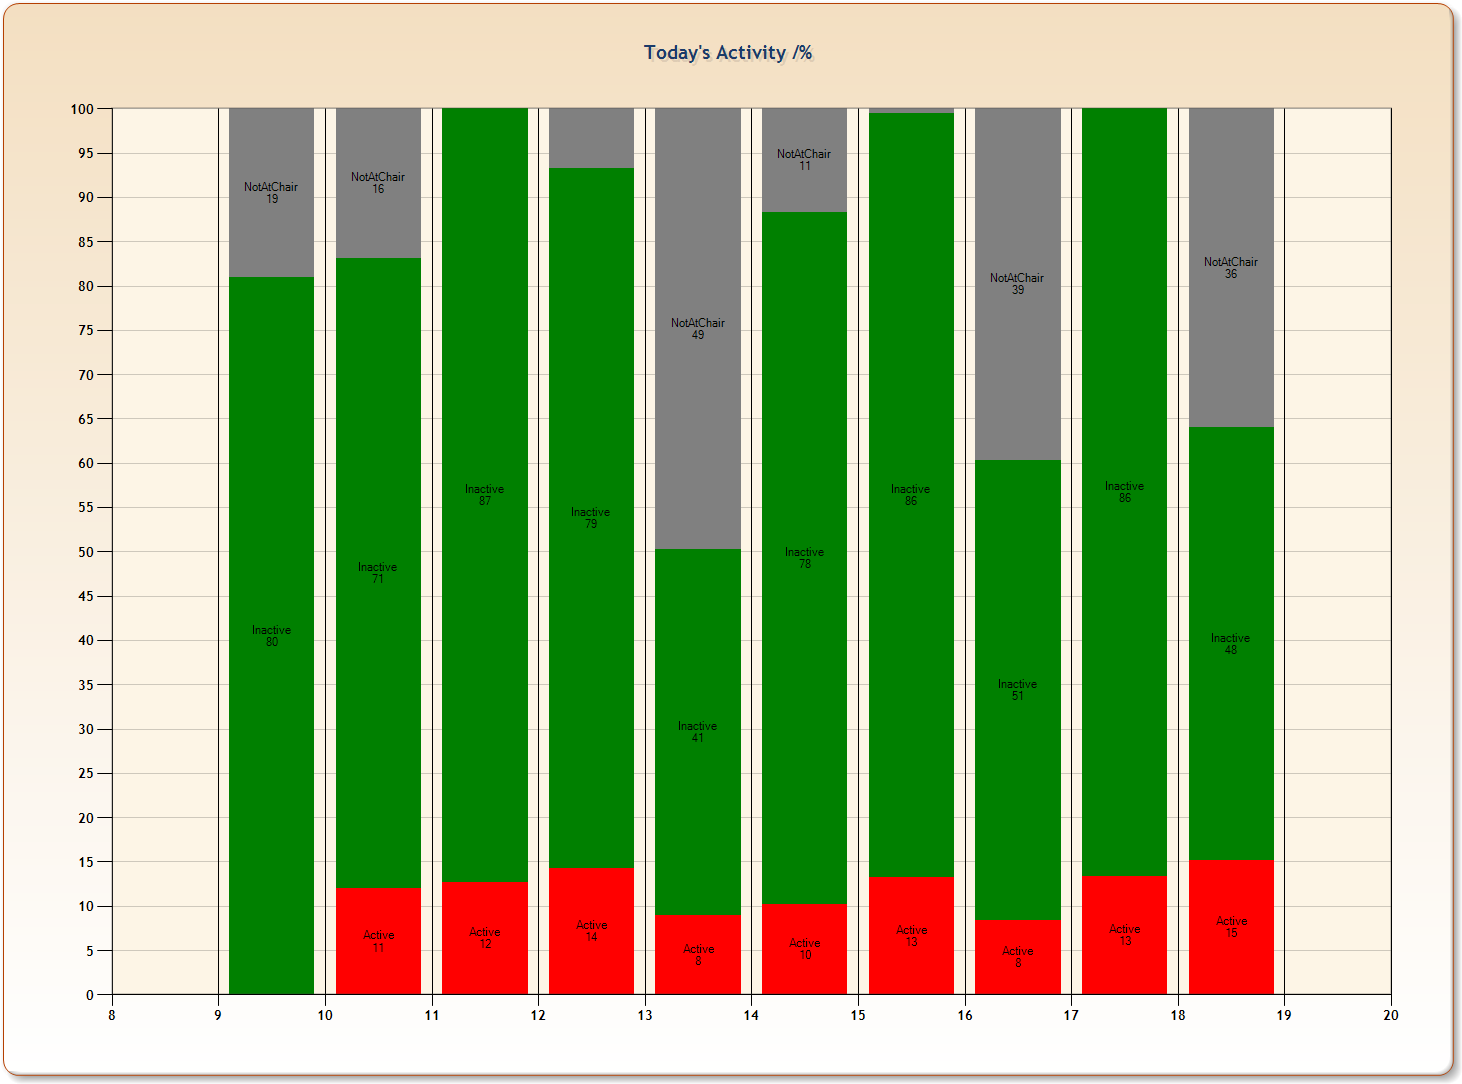
\includegraphics[width=0.8\textwidth]{images/prot_capchair_eval_work}
\captionof{figure}{Example chart of work activity data collected}
\label{fig:prot_capchair_eval_work}
\end{minipage}	

We can clearly see some phases of not at chair - usually for lunch break or some meetings and the work is distributed between active work, such as writing and typing and longer phases of inactivity (such as reading). More results can be found in Appendix \ref{ch:app_capchair_eval}.

\subsubsection*{Posture recognition}
In a second evaluation we were testing the posture recognition of the chair in a short study with 10 participants. Our system was tuned to distinguish three poses and a non-pose:
\begin{itemize}
\item Sitting upright
\item Sitting hunched
\item “Slouching on chair”
\item Close to chair - disturber
\end{itemize}

The persons were given a short introduction, the different postures were displayed, and finally the persons were asked to perform the postures in order. When testing “close-to-chair” the subjects were asked to rattle at the chair, stand close, move it around and thus disturb the potential sensor readings. Each class was tested for 10 seconds, collecting 200 samples. Overall the results were very convincing. Of the 40 different measurements series only two were not achieving 100\% accuracy. The Upright and Disturbance positions were classified correctly for all candidates. A single candidate had an 86\% rating on the hunched posture. A different candidate had a 55\% rating on the slouching position. The average of correctly classified postures is 98,5\%. Detailed results can be found in Appendix \ref{ch:app_capchair_eval}.


